\section{Computational Study\label{sec:experiments}}
We conduct a computational study to evaluate the performance of the proposed approach using real-world data from \hcunicamp. 
While the theoretical results provide guarantees on system stability, it is essential to assess the practical implications in a realistic setting.
To this end, we simulate the long-term surgery planning process and compare the proposed approach with a baseline policy in terms of patient waiting times and resource utilisation.

\subsection{Real-world Data\label{instances}}
The dataset comprises detailed information on surgery durations, operating theatre availability, team constraints, and specialty schedules over a one-year period (2025). 
Each month is treated as an individual instance of the operating theatre scheduling problem, while the full year is used to evaluate long-term system behaviour.

\subsection{Derivation of Model Inputs}
The data are processed to derive the inputs required for the strategic and operational components of the proposed approach.

\paragraph{\textbf{Surgery duration distributions}}
For each subspecialty, empirical distributions of surgery durations are estimated from historical data. 
These distributions are used in the Overtime and Cancellation module to evaluate the newsvendor model and determine the number of surgeries scheduled per block; see Section \ref{sec:module2}.

\paragraph{\textbf{Demand distributions}}
Patient arrivals are modelled as Poisson processes. 
For each subspecialty, the arrival rate $\lambda$ is estimated as the average monthly demand derived from historical activity.
%This is obtained by combining the expected number of surgeries per operating block (estimated from the duration distributions) with the observed number of allocated blocks, yielding an average monthly arrival rate.

\paragraph{\textbf{Operational parameters}}
All parameters of the operating theatre scheduling model (see Table~\ref{tab:symb} in Section~\ref{sec:ot}) are calibrated using real-world data, i.e., the actual values observed in each month of the year 2025.
These include operating theatre compatibilities, staff availability, and working calendars.

\subsection{Experimental Setup\label{sec:experimental_setup}}
Experiments are conducted on a machine equipped with an Intel Core 7 150U processor (5.40 GHz) and 32 GB of RAM. 
All modules are implemented in Python 3.12, and the MILP model is solved using SCIP 9.2.3 with default parameter settings, interfaced through the Pyomo library.

For the Queue Management module, the waiting time target is set to $\waittimereq = 6$ months with confidence level $\conflevel = 0.1$, ensuring that patients are treated within this horizon with high probability. 
The threshold $R$ is defined as the midpoint between $\lowq$ and $\upq$.

In the Overtime and Cancellation module, the overtime cost is set to twice the regular surgery cost, while the cancellation cost equals the regular cost. 
Additionally, we set the cost function to be quadratic in the number of surgeries cancelled, i.e., $c(x) = x^2$, reflecting the increasing marginal cost of cancellations as more surgeries are cancelled.

These strategic parameters are computed once and remain fixed throughout the simulation horizon.

\paragraph{\textbf{Baseline policy}}
The baseline policy excludes the strategic modules. 
All specialities are scheduled in every period, and the MILP model is solved using only operational constraints, without $(R,Q)$ control or overtime optimisation.
Essentially, we do so by deactivating the block demand constraints~\eqref{eq:c1} and~\eqref{eq:c2} in the MILP model and using the original surgery duration distributions (without adjustment for overtime or cancellations) to drawn the number of surgeries that happened into each scheduled block.
The patient arrival process and the operational parameters remain the same as in the proposed approach, ensuring a fair comparison.

\subsection{Simulation Framework}

Figure~\ref{fig:longterm_simulation} illustrates the simulation flow.
The system evolves over a monthly decision cycle.
In each period, patient arrivals are realised according to the estimated demand distributions, and queues are updated accordingly. 
Under the proposed approach, only specialties with queue size exceeding $R$ are selected for scheduling.

The MILP model then determines the allocation of operating theatre blocks. For the proposed approach, the number of surgeries is sampled based on the distributions obtained from the Overtime and Cancellation module. 
For the baseline policy, the number of surgeries is determined directly from surgery duration distributions without adjustment for overtime or cancellations.
Queues are updated after surgery, and the process repeats at each new period.

\begin{figure}[ht]
    \centering
    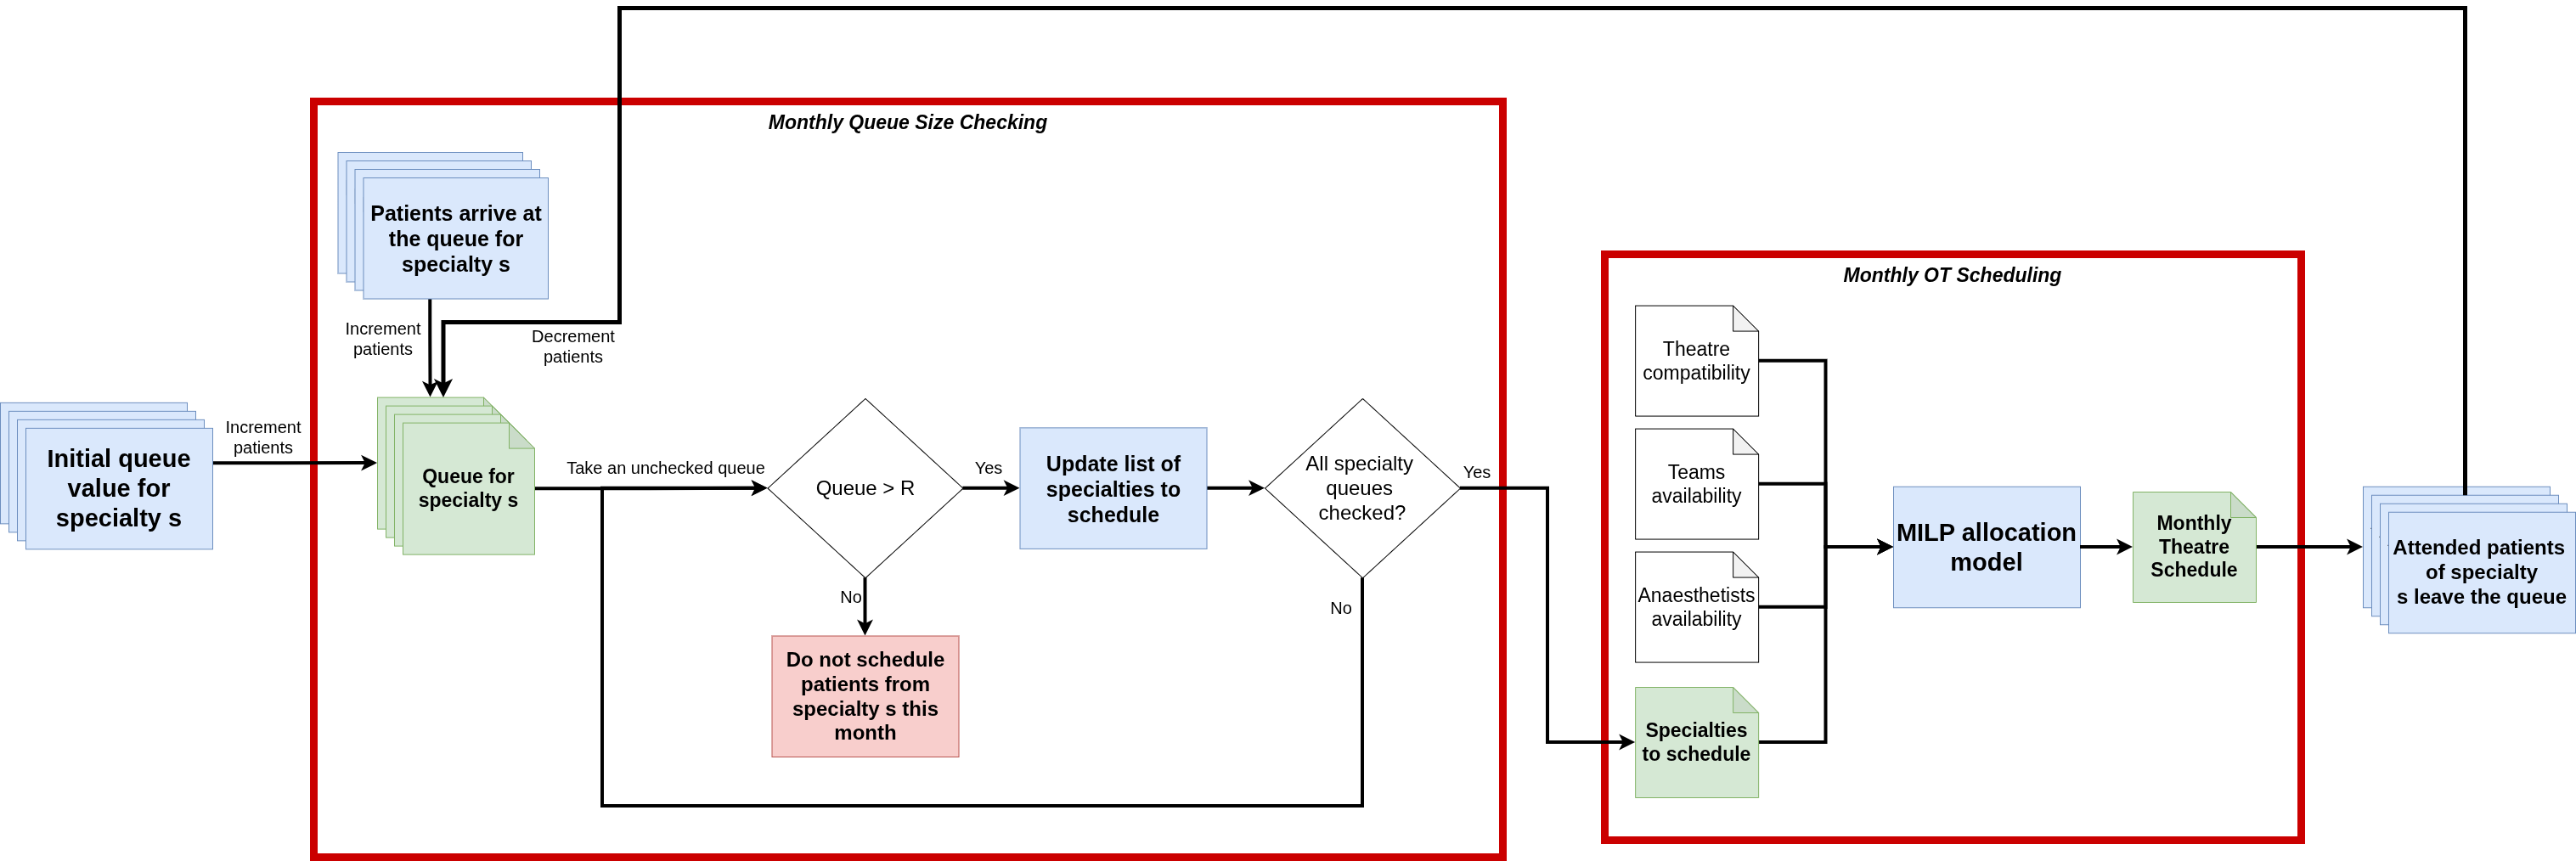
\includegraphics[width=0.9\textwidth]{images/experimental_design.png}
    \caption{Long-term simulation flow.}
    \label{fig:longterm_simulation}
\end{figure}

To assess long-term stability and the baseline, we perform $100$ independent simulation runs each, using different random seeds to capture the stochasticity in surgery durations and patient arrivals.

\subsection{Results from Strategic Decision-Making\label{sec:longterm_analysis}}

\subsubsection{$(R,Q)$ Policy Results}
% apresentar os tamanhos dos Q para cada especialidade (em numero de cirurgias)
% apresentar os tamanhos dos Q para cada especialidade (em numero de blocos)
% analise: quais especialidades tem Q mais altos? quais tem Q mais baixos? qual a relação entre Q e a demanda? qual a relação entre Q e o numero de blocos alocados? qual a relação entre Q e o tempo de espera dos pacientes?


\subsubsection{Overtime and Cancellation Results}
% apresentar resultados do newsvendor: 
% - o valor de t* para cada especialidade (tabela em apendice, talvez?)
% - grafico de distribuições de se planejar k cirurgias
% - analise: quais especialidades tem t* mais altos? quais tem t* mais baixos? talvez(relacao do t* com a distribuição do grafico); analisar o grafico e os impactos: quanto mais cirurgias planejar, maior a chande de cancelar (explicar intuitivamente)
% apresentar resultados do inventory-model:
% - grafico de custo vs ganho (uma ou duas especialidades)
% - analise: como isse modelo foi usado para definir um numero de otimo de cirurigas a planejar? por que ele é bom? qual o impacto do custo de overtime e cancelamento? qual o impacto da forma da função de custo (quadratica)?


\subsection{Long-term Stability Analysis\label{sec:otscheduling}}
In this section, we evaluate the long-term stability of the system under the proposed approach and compare it with the baseline policy.
We analyse the evolution of patient queues over time and the allocation of operating theatre blocks, highlighting the differences between the two approaches.

\subsubsection{Queue Management Results}
The one-year simulation horizon enables the analysis of queue dynamics under both the proposed framework and the baseline policy. 
As results are obtained from $100$ independent runs, we also assess variability through the 10--90\% percentile interval, which provides insight into the robustness of each approach.
\textcolor{red}{percebi que os graficos tem a mesma cor pro baseline e o proposto... todo: corrgir isso}

\begin{figure}[htb]
    \centering
    \begin{subfigure}[b]{0.45\textwidth}
        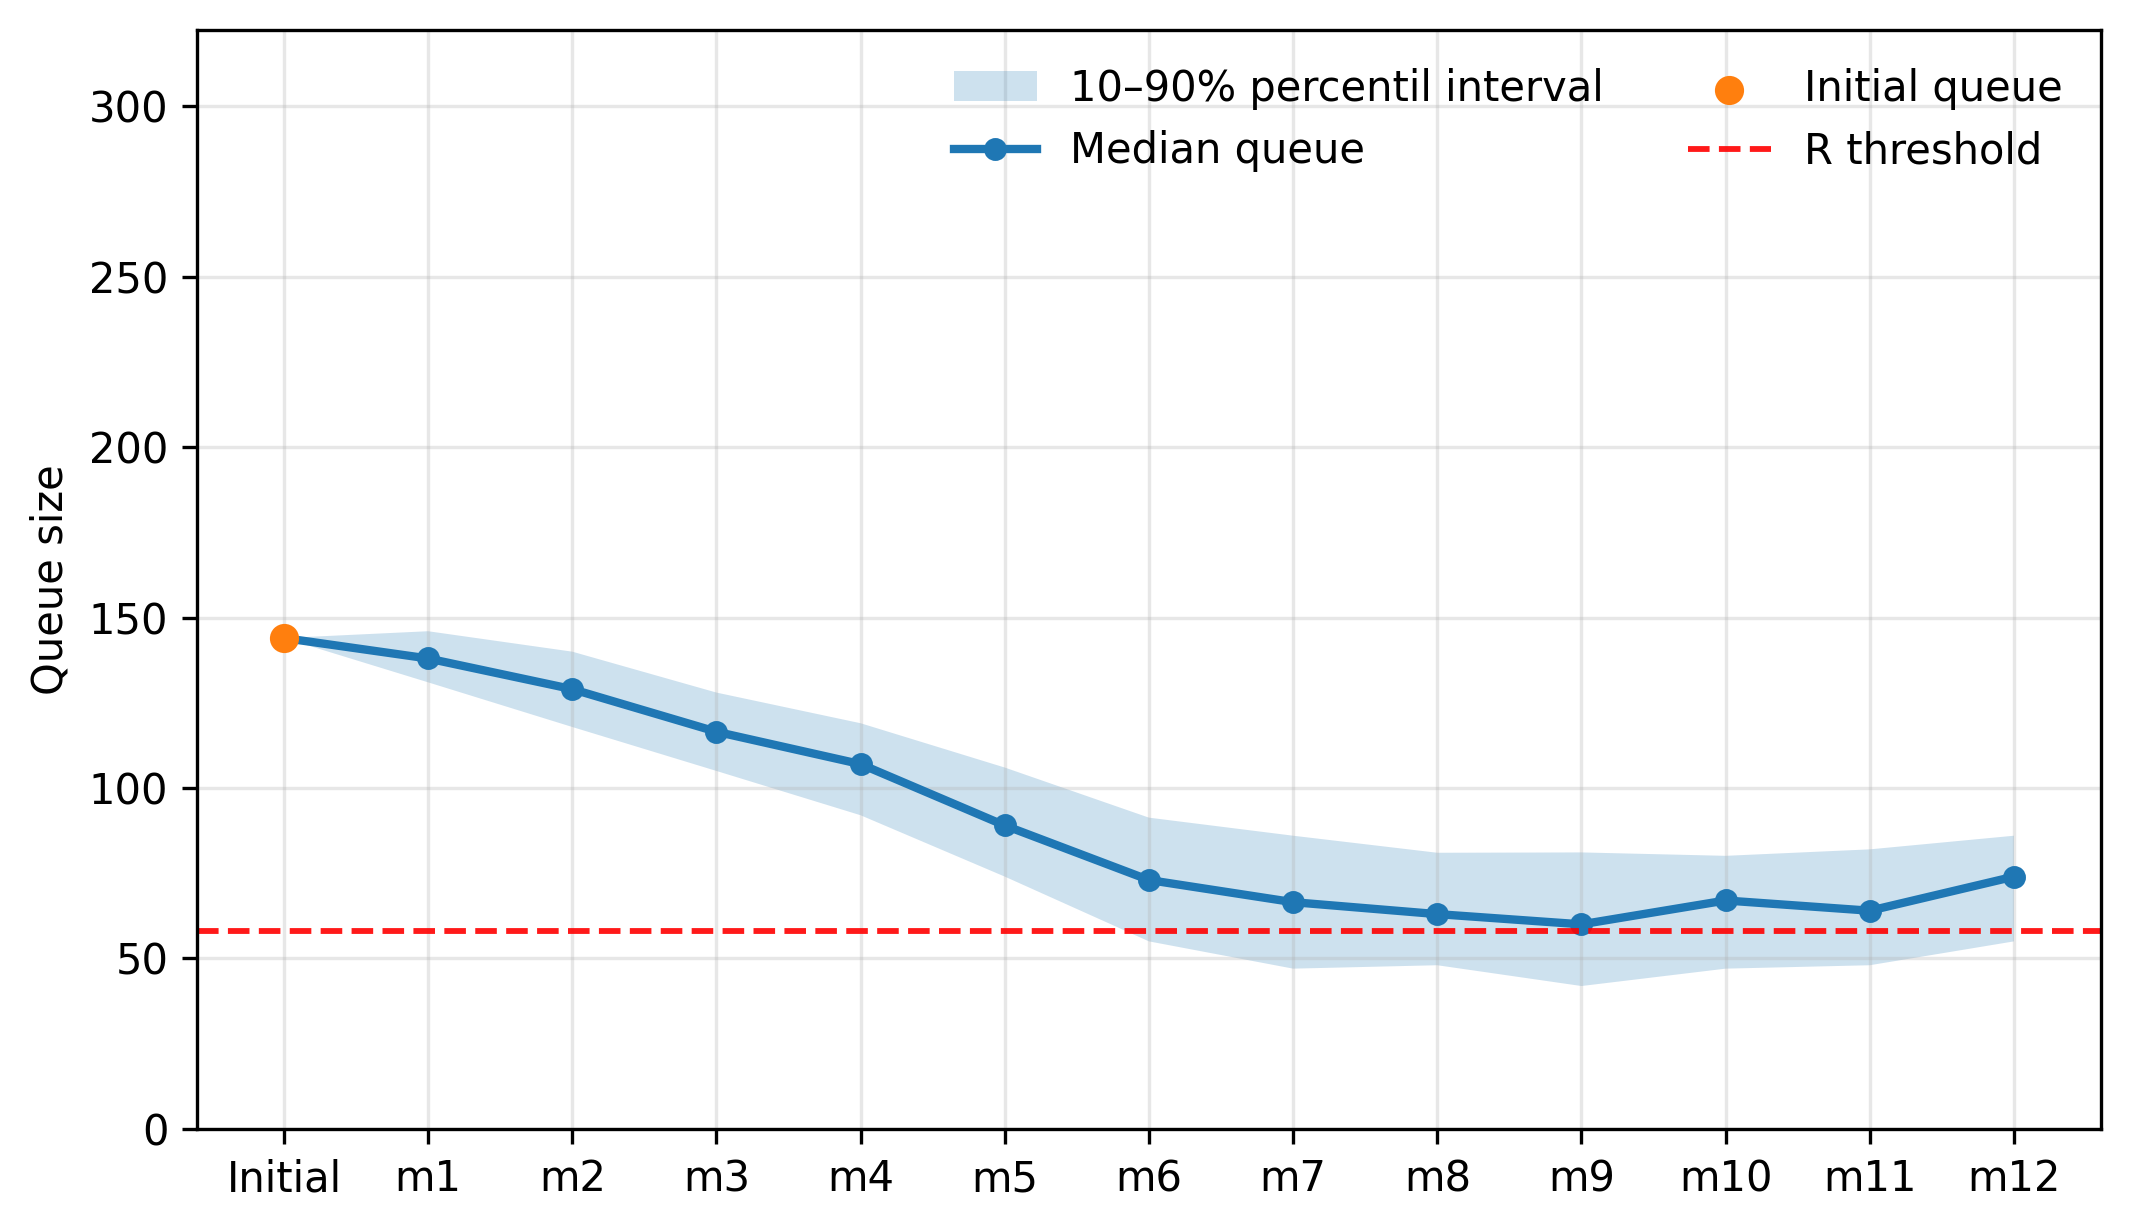
\includegraphics[width=\textwidth]{images/queue_trend_eda_infantil.png}
        \caption{Proposed approach.}
        \label{fig:eda_proposed}
    \end{subfigure}
    \hfill
    \begin{subfigure}[b]{0.45\textwidth}
        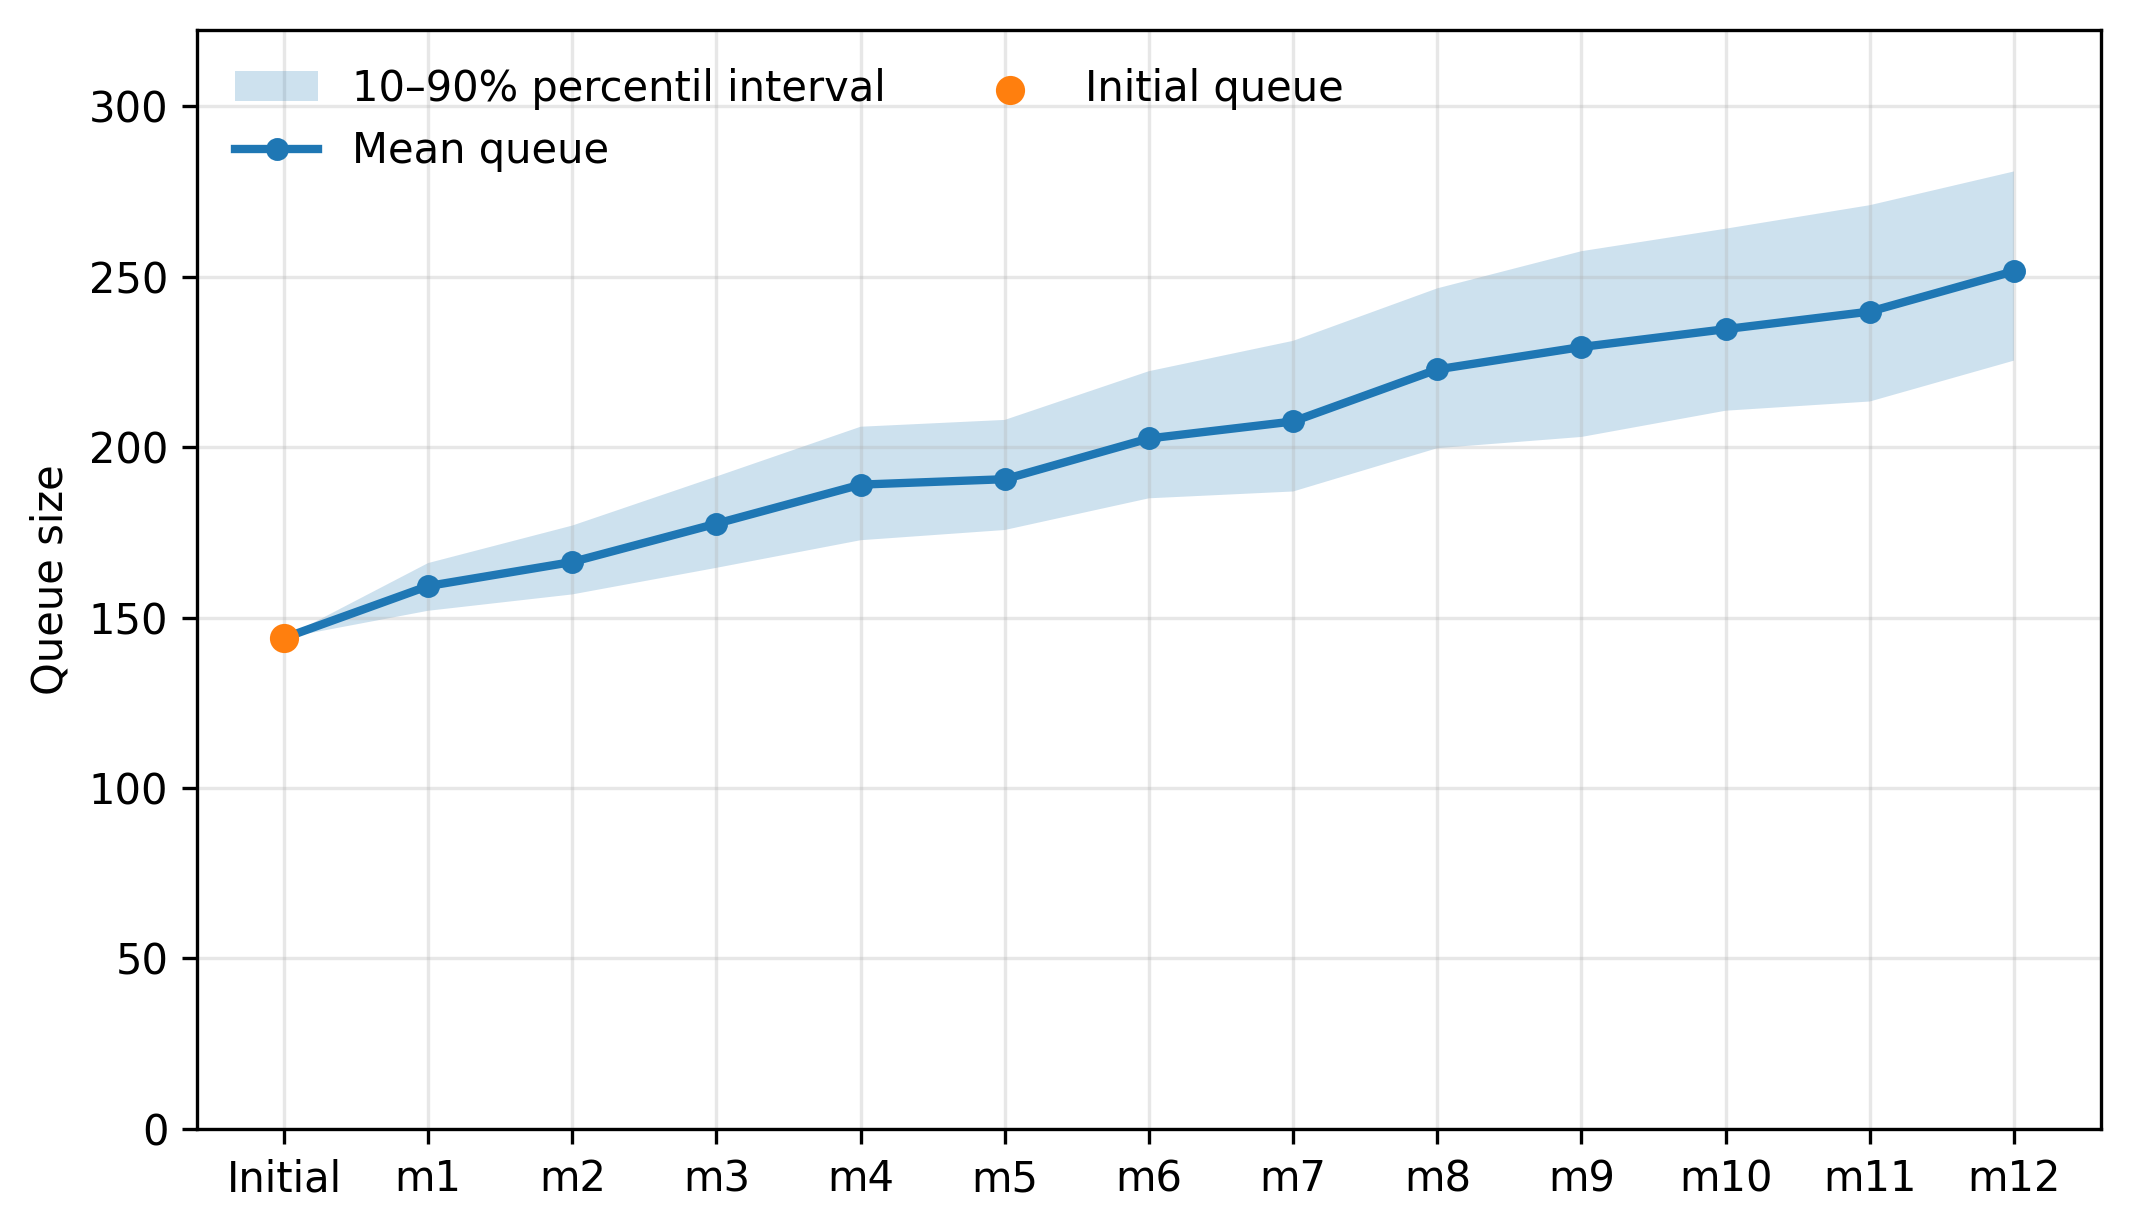
\includegraphics[width=\textwidth]{images/baseline_queue_trend_eda_infantil.png}
        \caption{Baseline policy.}
        \label{fig:eda_baseline}
    \end{subfigure}
    \caption{Evolution of patient queues over time for the subspecialty \textit{UDP -- Pediatric}.}
    \label{fig:queue_evolution_eda}
\end{figure}

Figure~\ref{fig:queue_evolution_eda} illustrates the evolution of the patient queue for the subspecialty \textit{Upper Digestive Endoscopy (UDP) -- Pediatric}. 
Under the proposed approach (Figure~\ref{fig:eda_proposed}), the queue exhibits a clear decreasing trend from the initial level, with variability gradually reducing over time. 
Once the queue approaches the threshold $R$ (around month 6--9), the policy implicitly limits further allocations to this subspecialty, allowing capacity to be redirected to others. 
As a result, the queue stabilises around the target level, avoiding both excessive backlog and unnecessary over-allocation.

In contrast, the baseline policy (Figure~\ref{fig:eda_baseline}) lacks any feedback mechanism based on queue size. 
Although an initial reduction is observed, the queue subsequently increases and displays a persistent upward trend, with widening variability. 
This indicates that the system is unable to regulate demand and capacity effectively, leading to potential instability and longer waiting times.

A similar behaviour is observed for the subspecialty \textit{Gastroenterology -- Esophagus-Stomach-Duodenum (ESD)} in Figure~\ref{fig:queue_evolution_gast_eed}. 
Under the proposed approach (Figure~\ref{fig:gast_proposed}), the queue decreases more rapidly than in the previous case, reflecting the higher service capacity available for this subspecialty. 
The queue then stabilises close to the threshold $R$, again indicating effective balancing between demand and allocation decisions.

\begin{figure}[ht]
    \centering
    \begin{subfigure}[b]{0.45\textwidth}
        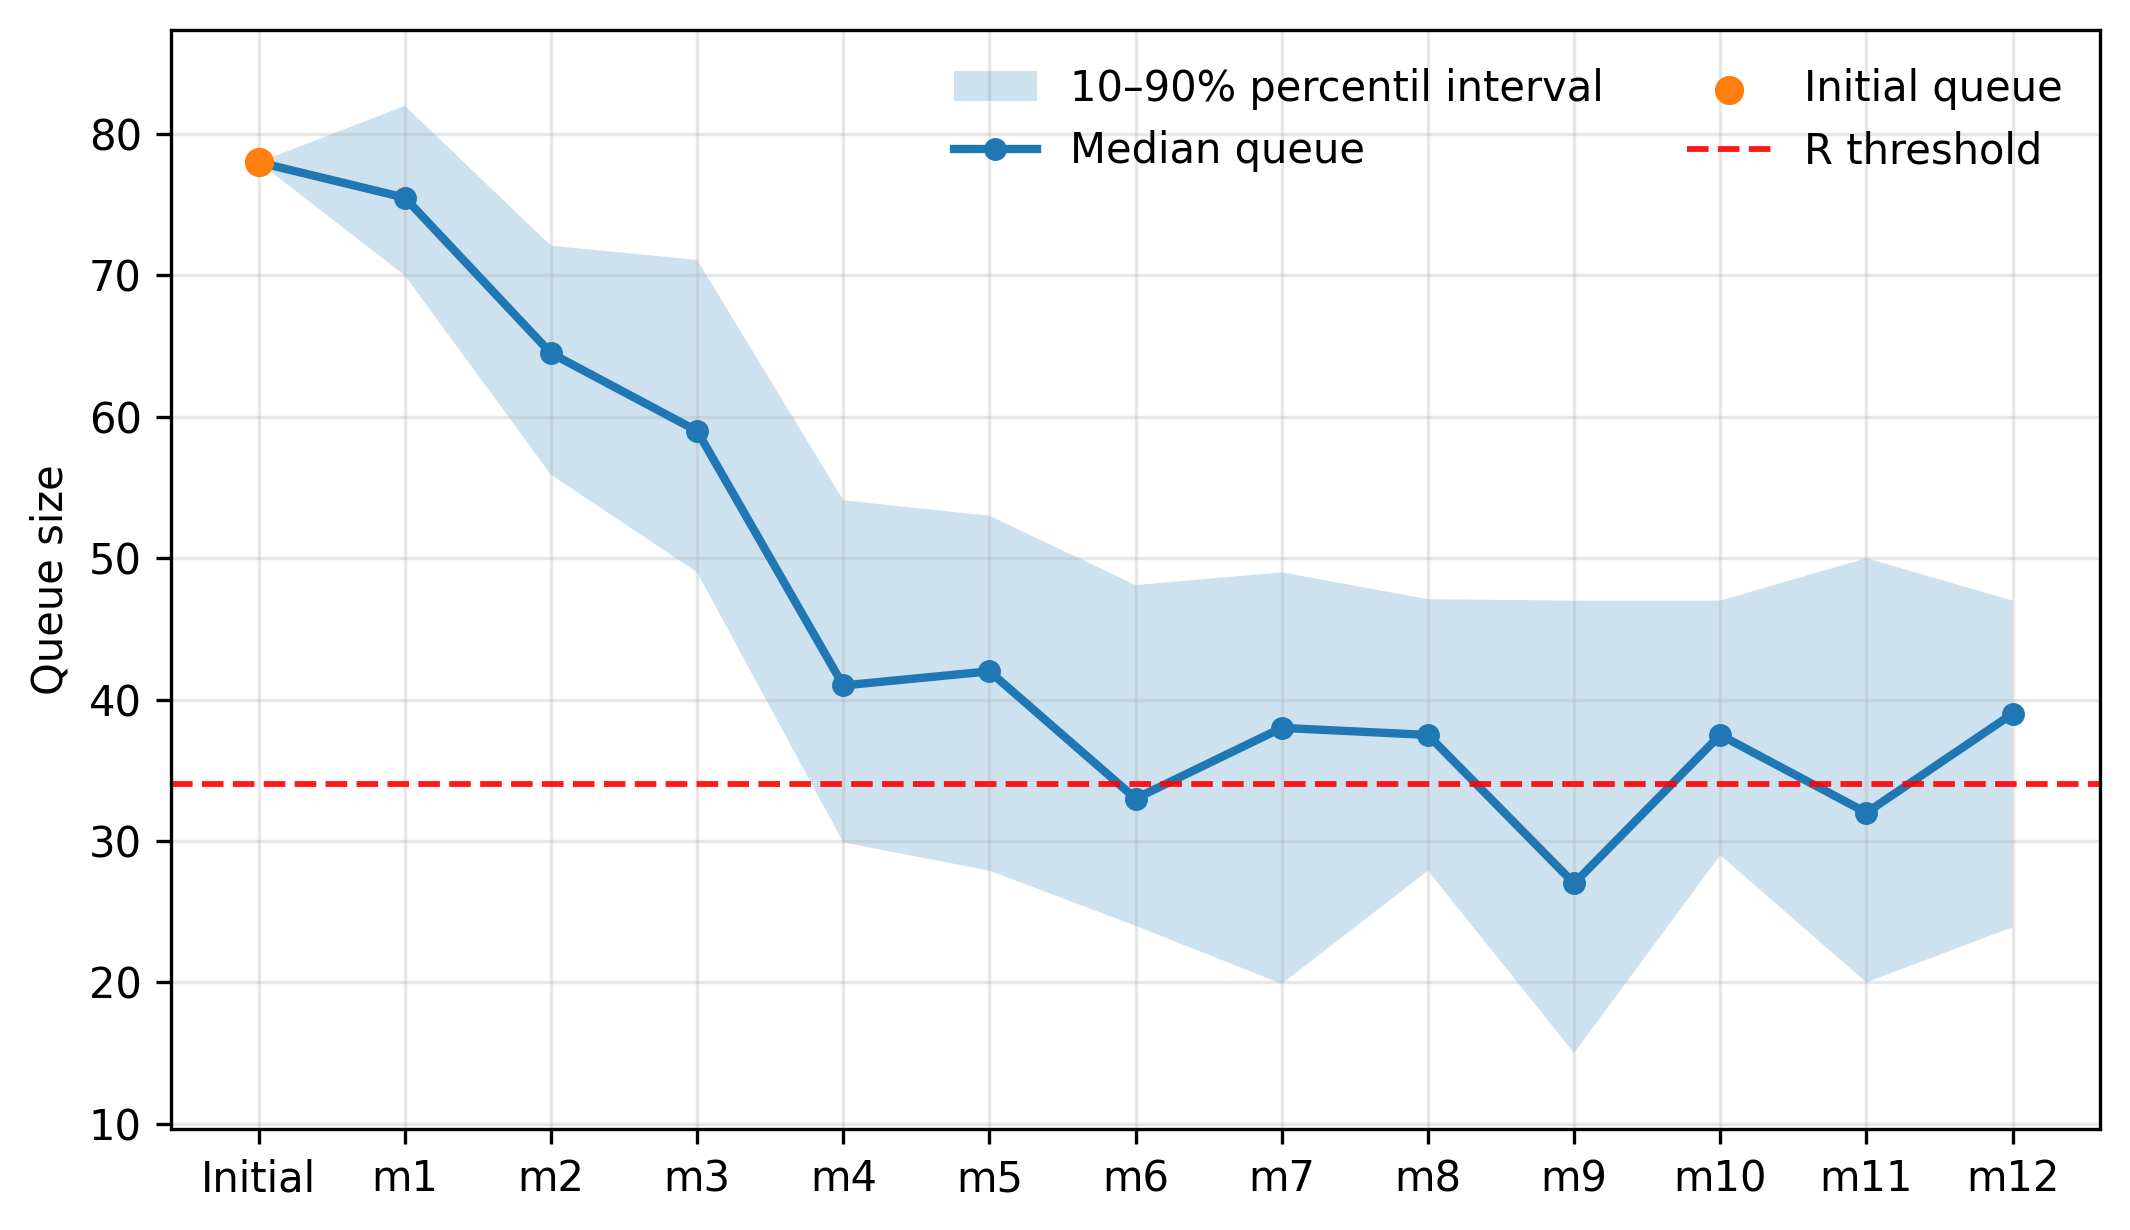
\includegraphics[width=\textwidth]{images/queue_trend_gast_eed.png}
        \caption{Proposed approach.}
        \label{fig:gast_proposed}
    \end{subfigure}
    \hfill
    \begin{subfigure}[b]{0.45\textwidth}
        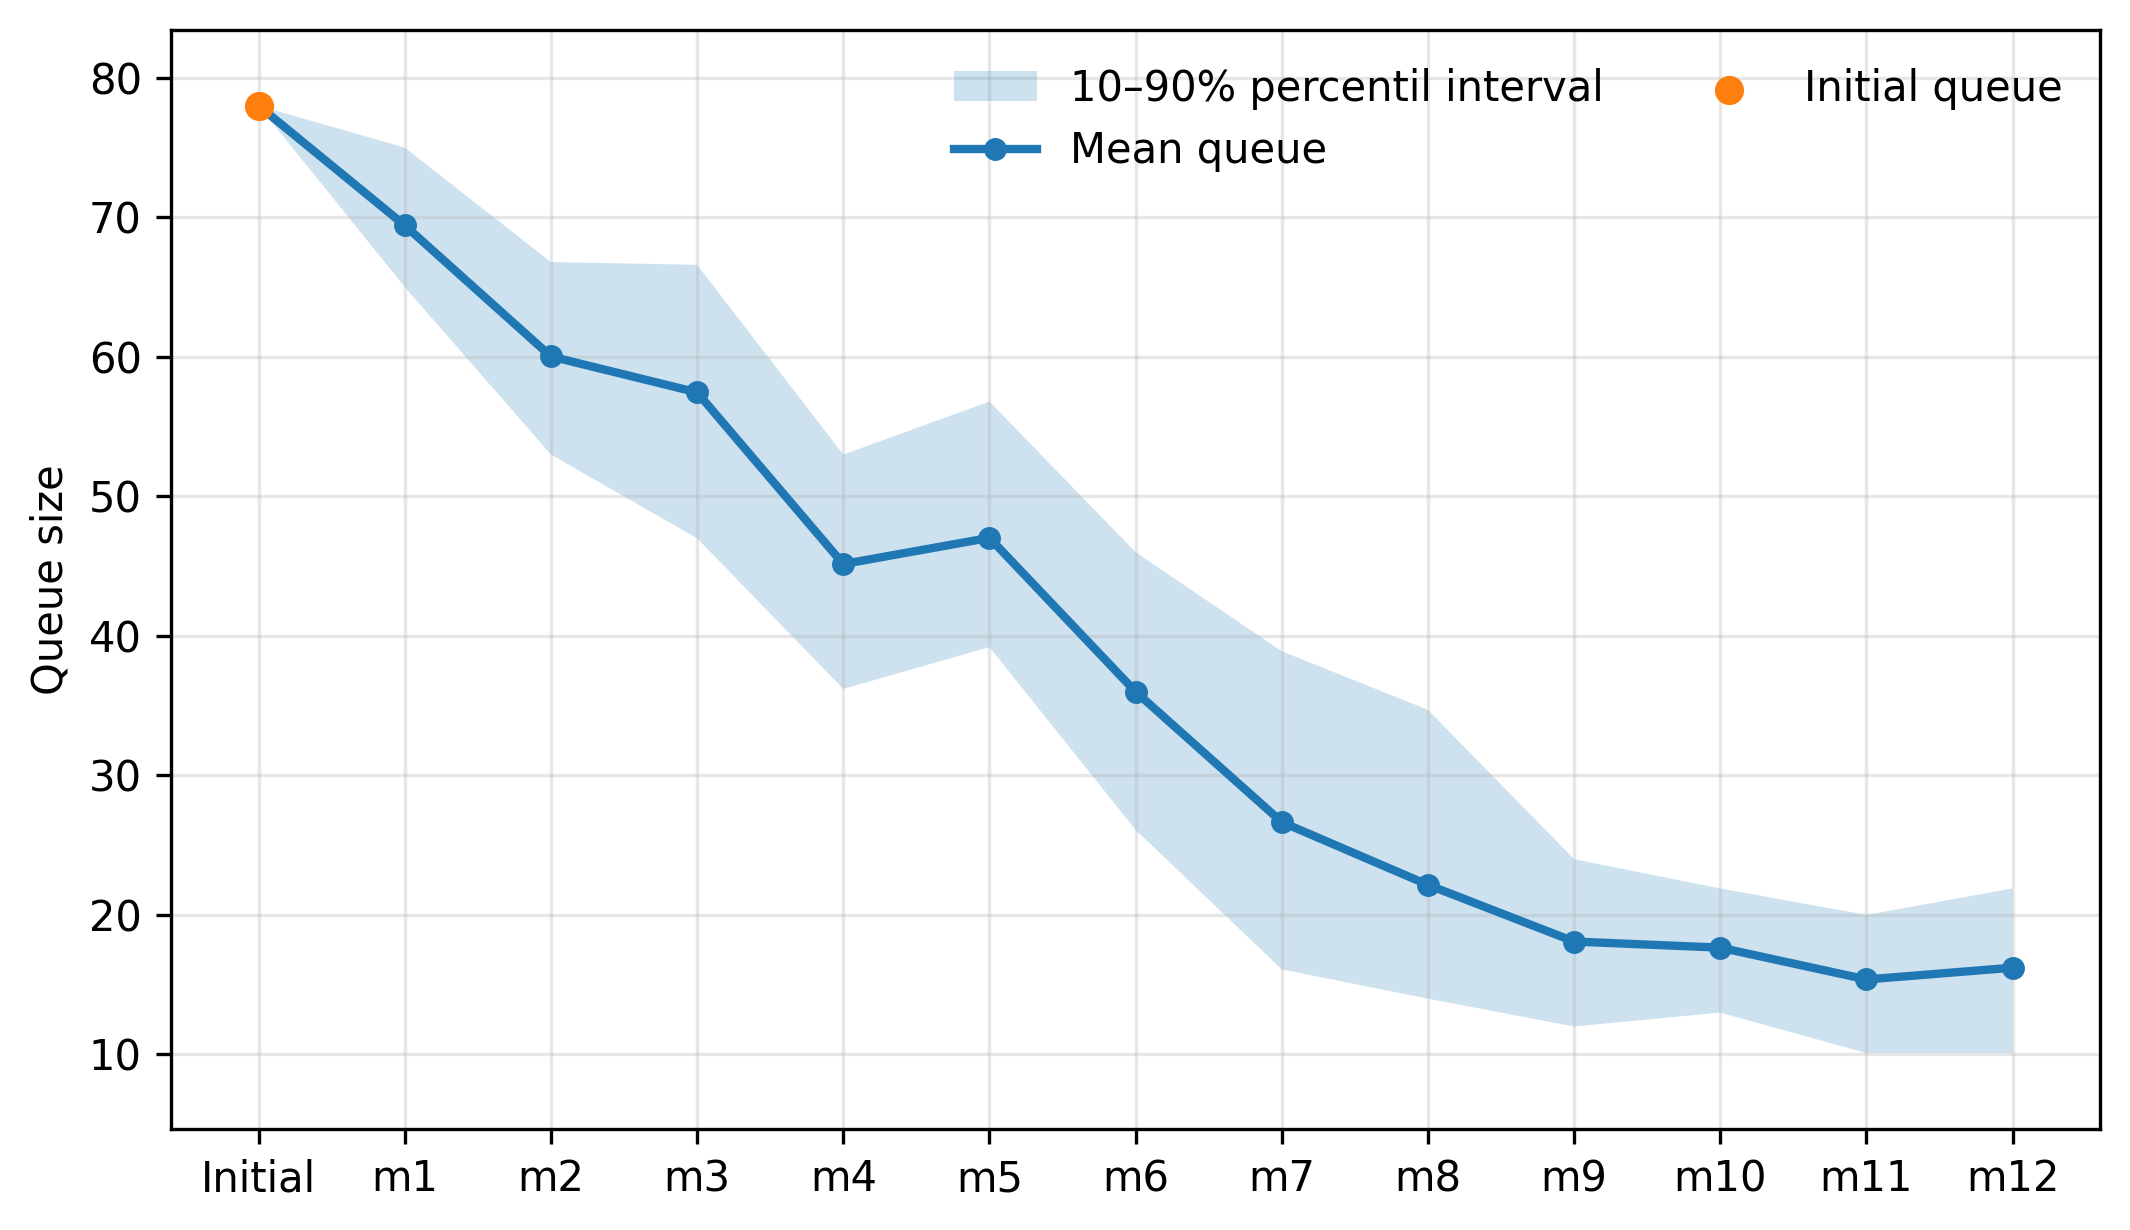
\includegraphics[width=\textwidth]{images/baseline_queue_trend_gast_eed.png}
        \caption{Baseline policy.}
        \label{fig:gast_baseline}
    \end{subfigure}
    \caption{Evolution of patient queues over time for the subspecialty \textit{Gastroenterology -- ESD}.}
    \label{fig:queue_evolution_gast_eed}
\end{figure}

For the baseline policy (Figure~\ref{fig:gast_baseline}), the queue also decreases over time, as this subspecialty is consistently allocated and benefits from sufficient capacity. 
However, this apparent improvement is misleading when viewed at the system level. 
Because the baseline allocates all subspecialties uniformly, without considering their relative queue sizes, it may over-serve some subspecialties (such as ESD) while neglecting others. 
This lack of awareness of queue dynamics can lead to imbalances across the system, even if individual queues appear well behaved.

These results show that the $(R,Q)$-based control introduces a feedback mechanism that regulates queue sizes around a target level, reduces variability, and promotes efficient use of capacity. 
In contrast, the baseline policy operates in an open-loop manner, which may lead to uncontrolled growth or inefficient allocation of resources. 
Detailed results for all subspecialties are provided in Appendix~\ref{app:queue_evolution}.

\subsubsection{OT Allocation Results}
% apresentar o grafico que mostra o quanto o framework alocou quando comparado ao intervalo Q (o grafico que brinquei que é ilícito -- só que melhorado)
% - discutir aqui que nossa abordagem nao aloca todas especialidades todo mes, o que dá vazao pra outras especialidades, aí dá pra mostrar dois graficos desse
% apresentar escalas mensais de alocação de sala